% Archivo generado automáticamente con los problemas
\section*{Problems}
Sección: 27_Gluon_scattering_and_the_spinor-helicity_formalism
Páginas: 578-579
Contenido:
27.1 What are the explicit polarization vectors ϵμ
± = 1
2σμ
α ˙αϵα ˙α
± when pμ = (E, 0, 0, E)
and rμ = (1, 0, 0, 1)? What would you choose rμ to be so that ϵμ = (0, 1, 0, 0) when
pμ = (E, 0, 0, E)?

27.2 Verify that the color-stripped amplitudes and Parke–Taylor formula reproduce the
gg →gg scattering cross section by using Eqs. (27.84) and (27.88) and adding the
appropriate color factors.

27.3 Prove the general formula for the matrix element in terms of color-ordered partial
amplitudes, Eq. (27.84).

27.4 Compute the Compton scattering cross section, γe−→γe−, in the high-energy
limit using helicity spinors. Check that you reproduce Eq. (13.141).

27.5 Calculate |M|2 summed over spins and colors for the remaining 2 →2 processes in
QCD. Fill out the following table:
560
Gluon scattering and the spinor-helicity formalism
Process
 |M|2/g4
s
Process
 |M|2/g4
s
q¯q →q′¯q′
4
9
t2+u2
s2
gg →gg
9
3(3 −tu
s2 −su
t2 −st
u2 )
qq′ →qq′
q¯q →gg
q¯q′ →q¯q′
gq →gq
qq →qq
gg →q¯q
q¯q →q¯q
where q and q′ refer to quarks of different flavor. The two entries shown come from
Eqs. (13.68) and (27.74).

27.6 Calculate the |M|2 summed over spins and colors for the process gg →ggg.

27.7 Prove the Parke–Taylor formula using BCFW recursion relations. If you do a couple
of cases (5-, 6- or 7-point amplitudes) you should see the pattern and the proof should
be straightforward.

27.8 In the proof of the Jacobi identity using factorization in Section 27.5.2, we chose a
particular pole, P 2 = 0, in the t-channel by taking [14] = 0 or ⟨14⟩= 0. Since
P 2 = ⟨23⟩[32] = ⟨14⟩[41] one also must choose ⟨23⟩= 0 or [23] = 0. Can you
derive any additional constraints on the form of the amplitude from considering all
four possible combinations, such as ⟨23⟩= [14] = 0 or ⟨23⟩= ⟨14⟩= 0?

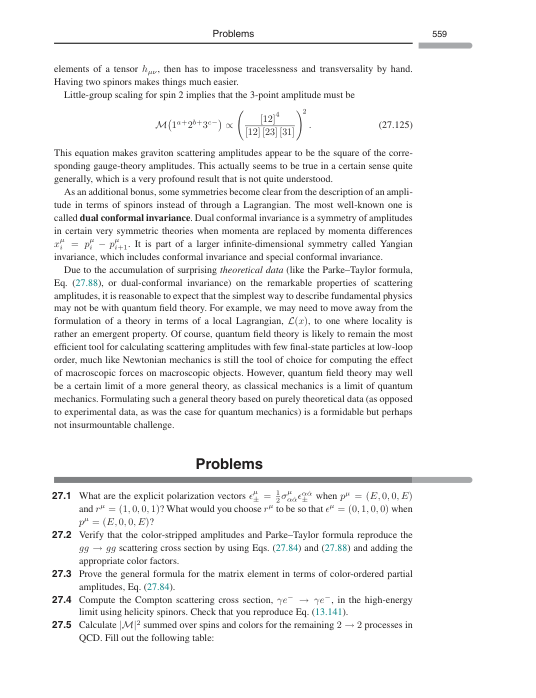
\includegraphics{./figs/27_Gluon_scattering_and_the_spinor-helicity_formalism_page_579.png}

---

